% Scalar instruction entry source: tools/generate_scalar_instruction_catalog.py.
\subsection{\texttt{BIC}}
\label{sec:scalar-bic}
\index{BIC@\texttt{BIC}}
\begin{sloppypar}\noindent\textbf{Purpose.} Bit clear / AND-NOT operation.\end{sloppypar}\smallskip
\noindent\textbf{Syntax.}\par
\begin{lstlisting}[style=ptoscalarcode]
bic SrcL, M, N, ->RegDst
\end{lstlisting}
\noindent\textbf{Encoding.}\par
\noindent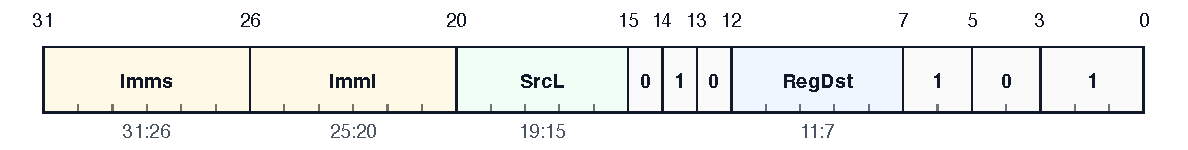
\includegraphics[width=\textwidth]{figs/encoding/scalar_instruction_entries/enc_bic.pdf}\par\smallskip
\begin{description}[leftmargin=0.18\linewidth,style=nextline]
\item[Format] \texttt{L32} \texttt{32-bit} scalar word.
\item[Pattern] \texttt{.................010.....1100111}.
\end{description}
\noindent\textbf{Classification.}\par
\begin{description}[leftmargin=0.18\linewidth,style=nextline]
\item[Category] Integer ALU and Bit-Manipulation.
\item[Family] Bit Operation.
\item[Execution class] \texttt{ALU}; uop\_kind=ALU.
\end{description}
\noindent\textbf{Operand fields.}\par
\begin{description}[leftmargin=0.18\linewidth,style=nextline]
\item[\texttt{RegDst}] Bits \texttt{11:7 (5b)}. 5-bit scalar destination register written by this instruction; X0 is hardwired to zero, so writes to X0 are ignored.
\item[\texttt{SrcL}] Bits \texttt{19:15 (5b)}. 5-bit scalar source register used as the left input operand.
\item[\texttt{imml}] Bits \texttt{25:20 (6b)}. 6-bit unsigned immediate operand consumed directly by the operation.
\item[\texttt{imms}] Bits \texttt{31:26 (6b)}. 6-bit unsigned immediate operand consumed directly by the operation.
\end{description}
\noindent\textbf{Operation.}\par
\begin{lstlisting}[style=ptoscalarcode]
mask = BitMask(M, N)
Write(RegDst, Read(SrcL) & ~mask)
\end{lstlisting}
\Needspace{0.08\textheight}
